\documentclass[ignorenonframetext,]{beamer}
\setbeamertemplate{caption}[numbered]
\setbeamertemplate{caption label separator}{: }
\setbeamercolor{caption name}{fg=normal text.fg}
\beamertemplatenavigationsymbolsempty
\usepackage{lmodern}
\usepackage{amssymb,amsmath}
\usepackage{ifxetex,ifluatex}
\usepackage{fixltx2e} % provides \textsubscript
\ifnum 0\ifxetex 1\fi\ifluatex 1\fi=0 % if pdftex
  \usepackage[T1]{fontenc}
  \usepackage[utf8]{inputenc}
\else % if luatex or xelatex
  \ifxetex
    \usepackage{mathspec}
  \else
    \usepackage{fontspec}
  \fi
  \defaultfontfeatures{Ligatures=TeX,Scale=MatchLowercase}
\fi
% use upquote if available, for straight quotes in verbatim environments
\IfFileExists{upquote.sty}{\usepackage{upquote}}{}
% use microtype if available
\IfFileExists{microtype.sty}{%
\usepackage{microtype}
\UseMicrotypeSet[protrusion]{basicmath} % disable protrusion for tt fonts
}{}
\newif\ifbibliography
\hypersetup{
            pdfborder={0 0 0},
            breaklinks=true}
\urlstyle{same}  % don't use monospace font for urls

% Prevent slide breaks in the middle of a paragraph:
\widowpenalties 1 10000
\raggedbottom

\AtBeginPart{
  \let\insertpartnumber\relax
  \let\partname\relax
  \frame{\partpage}
}
\AtBeginSection{
  \ifbibliography
  \else
    \let\insertsectionnumber\relax
    \let\sectionname\relax
    \frame{\sectionpage}
  \fi
}
\AtBeginSubsection{
  \let\insertsubsectionnumber\relax
  \let\subsectionname\relax
  \frame{\subsectionpage}
}

\setlength{\parindent}{0pt}
\setlength{\parskip}{6pt plus 2pt minus 1pt}
\setlength{\emergencystretch}{3em}  % prevent overfull lines
\providecommand{\tightlist}{%
  \setlength{\itemsep}{0pt}\setlength{\parskip}{0pt}}
\setcounter{secnumdepth}{0}
\usepackage[orientation=portrait,size=a0]{beamerposter}
\title{Rmarkdownでポスター発表用のポスターを作成する}
\author{NAKAJIMA Yukihiro}
\institute{Rmarkdown大学 \LaTeX 学部}
\usepackage{luatexja}
\usepackage[ipaex]{luatexja-preset}
\renewcommand{\kanjifamilydefault}{\gtdefault}
\usetheme{sumiilab-poster}
\beamertemplatenavigationsymbolsempty
\renewcommand{\figurename}{図}
\renewcommand{\tablename}{表}
\def\bcols{\begin{columns}}
\def\bcol{\begin{column}}
\def\ecol{\end{column}}
\def\ecols{\end{columns}}
\def\bblck{\begin{block}}
\def\eblck{\end{block}}
\usepackage{tikz}
\usetikzlibrary{positioning}
\newcommand{\highlightcap}[3][yellow]{\tikz[baseline=(x.base)]{\node[rectangle,rounded corners,fill=#1!10](x){#2} node[below of=x, color=#1]{#3};}}

\date{}

\begin{document}

\begin{frame}

\bblck{ポスターをRmarkdownで}
Rmarkdownを使って、ポスターを描くことができます。
ポスターをRmarkdownで書くことの利点は様々挙げられますが、主な理由は以下の通りです。

Rmarkdownでポスターを書いた方がいい理由

\begin{itemize}
\tightlist
\item
  すぐに研究を再現できる
\item
  スライドで発表した資料などを使いまわせる
\item
  キレイ
\item
  パワーポイントにはアレルギーがある

  \begin{itemize}
  \tightlist
  \item
    Officeが苦手な方はぜひ!
  \end{itemize}
\end{itemize}

\eblck

\bcols[onlytextwidth]
\bcol{0.495\textwidth}

\bblck{表を書いてみる}

アヤメの花(iris)のデータ(Anderson 1936; FISHER
1936)を使って色々書いてみましょう。 表
\ref{head}には、irisの上から5行を表示しています。

\begin{table}[ht]
\centering
\caption{irisの上から6行を例示} 
\label{head}
\scalebox{0.95}{
\begin{tabular}{rrrrl}
  \hline
Sepal.Length & Sepal.Width & Petal.Length & Petal.Width & Species \\ 
  \hline
5.10 & 3.50 & 1.40 & 0.20 & setosa \\ 
  4.90 & 3.00 & 1.40 & 0.20 & setosa \\ 
  4.70 & 3.20 & 1.30 & 0.20 & setosa \\ 
  4.60 & 3.10 & 1.50 & 0.20 & setosa \\ 
  5.00 & 3.60 & 1.40 & 0.20 & setosa \\ 
   \hline
\end{tabular}
}
\end{table}

\eblck

\bblck{表を書いてみる}

図 \ref{fig:Petal_plot}は花弁の長さと幅の散布図を示しています。

\begin{figure}
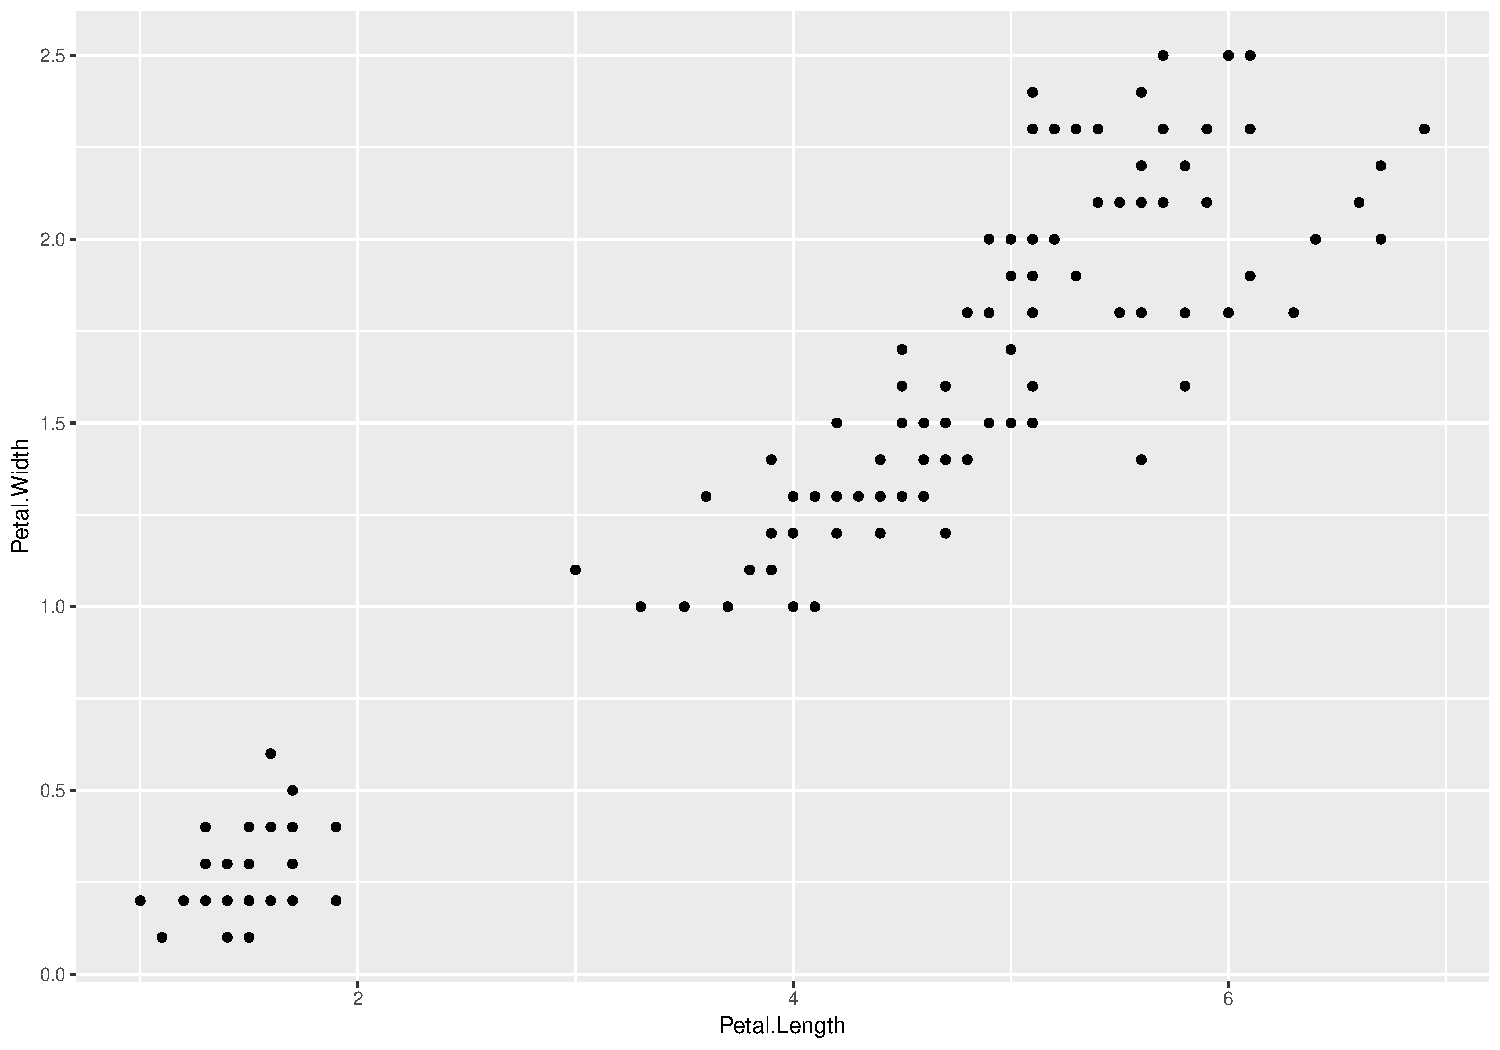
\includegraphics[width=\textwidth]{Rmd2BeamerPoster_files/figure-beamer/Petal_plot-1} \caption{花弁の長さと幅の散布図}\label{fig:Petal_plot}
\end{figure}

\eblck

\ecol
\bcol{0.495\textwidth}

\bblck{数式を書いてみる}

少し複雑な式を書いてみましょう。
式\ref{cor}にピアソンの積率相関係数を求める式を書いてみました。
パワーポイントなどで数式を書くのは大変ですが、
\LaTeX 記法ならきれいに一発で書けますね。

\begin{align}
r_{xy} = \dfrac{\Sigma_{i=1}^n (x_i-\overline{x})(y_i-\overline{y})}
            {\sqrt{\Sigma_{i=1}^n (x_i-\overline{x})^2}
             \sqrt{\Sigma_{i=1}^n (y_i-\overline{y})^2}}
\label{cor}
\end{align}

\eblck

 

\bblck{表の中で特殊文字を書いてみる}

表の中でギリシャ文字などの特殊文字を書きたいことがあると思います。

まず、式\ref{lm}を利用して回帰分析をしましょう。

\begin{align}
y = \highlightcap[red]{$\alpha$}{切片}
    +
    \highlightcap[blue]{$\beta$}{回帰係数}
    \highlightcap[blue]{$X$}{説明変数}
    +
    \highlightcap[green]{$\varepsilon$}{誤差項}
\label{lm} 
\end{align}\begin{align}
\varepsilon \sim N(0, \sigma^2) \label{epsilon}
\end{align}

\(y\)は花弁の幅、\(X\)は花弁の長さとして分析します。
InterceptやPepal.Lengthではなく、\(\alpha\)や\(\beta\)として出力してみましょう。
その結果が、表\ref{lm_table}です。

\begin{table}[ht]
\centering
\caption{回帰分析の結果} 
\label{lm_table}
\scalebox{0.95}{
\begin{tabular}{rrr}
  \hline
 & 回帰係数 & P値 \\ 
  \hline
$\alpha$ & -0.363 & 0.000 \\ 
  $\beta$ & 0.416 & 0.000 \\ 
   \hline
\end{tabular}
}
\end{table}

自由度調整済み決定係数は0.93でした。

\eblck

\ecol
\ecols

引用文献

\small

\hypertarget{refs}{}
\hypertarget{ref-Anderson1936}{}
Anderson, Edgar. 1936. ``The Species Problem in Iris.'' \emph{Annals of
the Missouri Botanical Garden} 23 (3):
457--469+471--483+485--501+503--509.
doi:\href{https://doi.org/10.2307/2394164}{10.2307/2394164}.

\hypertarget{ref-Fisher1936}{}
FISHER, R. A. 1936. ``THE USE OF MULTIPLE MEASUREMENTS IN TAXONOMIC
PROBLEMS.'' \emph{Annals of Eugenics} 7 (2). Blackwell Publishing Ltd:
179--88.
doi:\href{https://doi.org/10.1111/j.1469-1809.1936.tb02137.x}{10.1111/j.1469-1809.1936.tb02137.x}.

\end{frame}

\end{document}
